\section{Theorie}
\label{sec:Theorie}
Dieses Experiment befasst sich mit der Bestimmung der Brechungsindices
von Gasen und Festkörpern mittels Sagnac-Interferometer.

%\subsection{Interferenz}
\subsection{Das Sagnac-Interferometer}
Das Sagnac-Interferometer ist aufgebaut wie in Abbildung \ref{fig:apparat}.
\begin{figure}
    \centering
    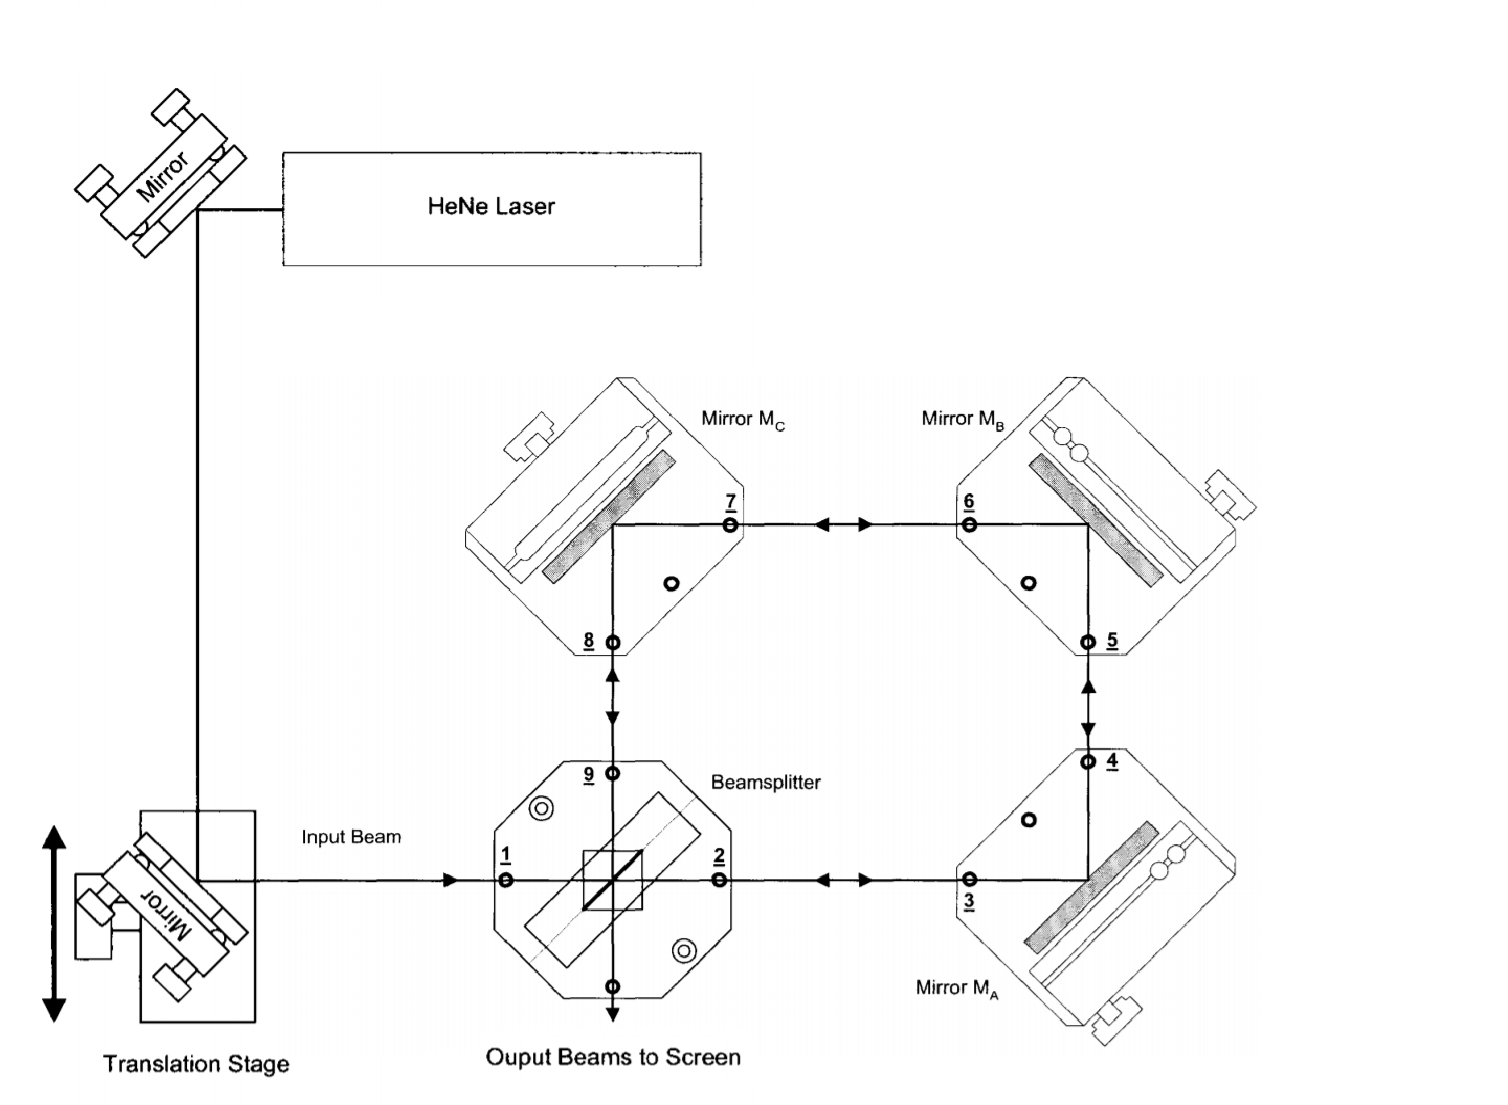
\includegraphics[width=0.7\textwidth]{Apparatur.PNG}
    \caption{Aufbau des Sagnac-Interferometers.\cite{skript}}
    \label{fig:apparat}
\end{figure}
\FloatBarrier
Die Anordnung setzt sich zu Beginn zusammen aus der Quelle, einem HeNe-Laser, der linear polarisiertes Licht emittiert, und zwei
Spiegeln zur Ausrichtung des Laserstrahls zum Polarizing-Beam-Splitter-Cube hin.
Der PBSC dient zur Aufspaltung des Strahls in Horizntal- und Vertikalkomponente,
dabei passiert die Horizontalkomponente den PBSC und die Vertikalkomponente
erfährt eine Richtungsänderung um $90\si{\degree}$. Dies ist in der Abbildung
\ref{fig:pbsc} dargestellt.
\begin{figure}
   \centering
   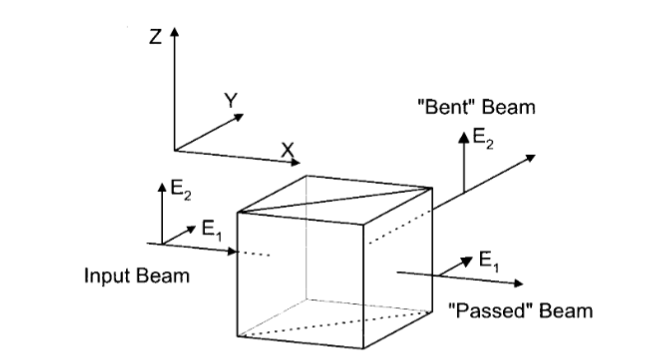
\includegraphics[width=0.7\textwidth]{Pbsc.PNG}
   \caption{Aufaspaltung des Strahls im PBSC.\cite{skript}}
   \label{fig:pbsc}
\end{figure}

Drei weitere Spiegel lenken beide Strahle so um, dass diese die gleiche Strecke zurücklegen und wieder auf
den PBSC treffen.
Dort werden die zuvor aufgespaltenen Strahlen erneut durchgelassen bzw. umgelenkt, je nach Polarisationszustand.
Der horizontalpolarisierte Strahl wird durchgelassen und der vertikalpolarisierte Strahl abgelenkt, dadurch laufen sie
wieder zuammen.
Durch Verschieben der Translation-Stage können die zwei Strahlen im Interferometer räumlich separiert
werden und somit zwei unterschiedliche Materialien durchqueren.

\FloatBarrier

\subsection{Brechungsindices von Gasen}
Für die Bestimmung von Brechungsindices von Gasen wird eine Gaszelle
der Länge $L$ genutzt. Einer der Strahlen passiert dabei die Gaszelle.
Ändert sich der Druck innerhalb der Gaszelle, so ändert sich auch
der Brechungsindex des Gases. Dies erzeugt eine Phasenverschiebung:
\begin{align}
  \Delta\phi=\frac{2\pi}{\lambda_\mathrm{vac}}(n-1)L.
\end{align}
Durch diese Phasenverschiebung entstehen Interferenzerscheinungen.
Die dabei zählbaren Extrema $M$ sind in folgender Beziehung abhängig
vom Brechungsindex $n$:
\begin{align}
  M=\frac{n-1}{\lambda_\mathrm{vac}}L\label{eqn:gas}.
\end{align}

\subsection{Brechungsindices von Festkörpern}
Zur Bestimmung des Brechungsindex wird eine dünne transparente
Platte des Festkörpers mit der Breite $T$ genutzt. Diese wird senkrecht in einen der Strahlengänge
platziert und in der Horizontalebene mit dem  Winkel $\theta$, der den Winekl zwischen der Startposition und der Platte angibt, ausgelenkt. Somit wird die
Strecke, die der Strahl in dem Festkörper zurücklegt, ebenfalls kontinuierlich größer.
Es entsteht wieder eine Interferenzerscheinung.
Es lässt sich eine Beziehung zwischen den zählbaren Extrema $M$
und dem Brechungsindex $n$ herleiten:
\begin{align}%1/(1-M*lam/(T*theta**2))
  n&=\frac{\alpha^2+2(1-\cos\theta)(1-\alpha)}{2(1-\cos\theta-\alpha)}\\
  \text{mit} \ \ \alpha&= \frac{M\lambda_\mathrm{vac}}{2T}. \label{eqn:glas}
  % \intertext{}
  % n&\approx \frac{1}{1-\frac{M\lamda_\mathrm{vac}}{T*\theta^2}
\end{align}
